\section{\texorpdfstring{Phương pháp nghiên cứu}{Method}}
\subsection{\texorpdfstring{Phương pháp đánh giá kết quả nghiên cứu}{Empty}}
Dựa vào từng loại bài toán giải quyết mà có những cách đánh giá khác nhau. Do tính chất của bài toán truy tìm đối tượng dựa vào thuộc tính cho dãy camera quan sát, có tính phân loại đúng sai nhiều nhãn. Tức là khi cho một đầu vào là một tấm hình chứa người đi bộ, model sẽ phân tích và gán nhãn cho tấm hình này có những thuộc tính nào, từ đó hỗ trợ cho việc truy vấn bằng các thuộc tính. Các thuộc tính gán nhãn này có thể đúng hoặc sai. Vì vậy, tác giả sử dụng các thông như sau để đánh giá mô hình.\\

\textit{Mean Accuracy - mA}: Được định nghĩa theo công thức sau 

\begin{equation}
mA = \frac{1}{2N} \sum_{i=1}^{L} (\frac{TP_i}{P_i} + \frac{TN_i}{N_i})
\end{equation}
\indent{}Trong đó:

\indent{}\indent{}$N$: số mẫu dự liệu trong tập dữ liệu

\indent{}\indent{}$L$: số thuộc tính trong tập dữ liệu 

\indent{}\indent{}$TP_i$: True Positive của thuộc tính thứ $i$

\indent{}\indent{}$P_i$: Positive của thuộc tính thứ $i$

\indent{}\indent{}$TN_i$: True Negative của thuộc tính thứ $i$

\indent{}\indent{}$N_i$: Negative của thuộc tính thứ $i$\\

\textit{Accuracy - Accu}: Được định nghĩa tỉ lệ mẩu dữ liệu được dự đoán đúng trên tất cả tổng tất cả các mẫu dự liệu được dự đoán. Trong trường hợp lý tưởng, $Accuracy$ càng cao thể hiện model dự đoán càng tốt. Tuy nhiên, có một nhược điểm khi dùng $Accuracy$ trong trường hợp dữ liệu không cân bằng giữa các lớp. Vì thế, $Accuracy$ không phải là độ đo khách quan để đánh giá.\\

\textit{Precision - Prec}: Được định nghĩa là tỉ lệ số điểm true positive trong số những điểm được phân loại là positive

\begin{equation}
Precision = \frac{TP}{TP + FP}
\end{equation}
\indent{}Trong đó:

\indent{}\indent{}$TP$: True Positive

\indent{}\indent{}$FP$: False Positive\\

\textit{Recall}: Được định nghĩa là tỉ lệ số mẫu true positive trong những mẫu số thực sự là positive.

\begin{equation}
Recall = \frac{TP}{TP + FN}
\end{equation}

\indent{}Trong đó:

\indent{}\indent{}$TP$: True Positive

\indent{}\indent{}$FP$: False Negative\\

\textit{F1 score - F1}: $F_1$ score là trung bình điều hòa của $Precision$ và $Recall$, có giá trị nằm trong khoảng $(0, 1]$. Vì thế $F_1$ là một thang đo cân bằng, không bị ảnh hưởng bởi mật độ cân bằng từ dữ liệu, cũng như mật độ từ các dữ liệu mất cân bằng. Cũng vì chính lý do này, $F_1$ là một thước đo đáng tin cậy trong mô hình phân lớp.

\begin{equation}
F_1 = 2 * \frac{Precision * Recall}{Precision + Recall}
\end{equation}



\subsection{\texorpdfstring{Phương pháp thu thập và phân tích số liệu}{Empty}}
Về mặt dữ liệu, tác giả kế thừa và sử dụng các tập dữ liệu có sẵn và được thử nghiệm trên các mô gần đây. Các tập dữ liệu sau được thử nghiệm trong luận văn này:

\textit{PA-100K}[\ref{refer:1}]: Bao gồm 100000 ảnh người đi bộ có độ phận giải từ 50x100 đến 758x454 được thu thập từ các camera ngoài trời. Tập dữ liệu này có 26 thuộc tính và được chia thành 3 phần: 80000 cho tập huấn luyện, 10000 ảnh cho tập kiểm thử, 10000 ảnh cho tập kiểm tra.

\textit{PATE}[\ref{refer:2}]: Bao gồm 19000 ảnh người đi bộ có độ phân giải từ 17x39 đến 169x365 được tổng hợp từ 10 nguồn dữ liệu nhỏ sau đó loại bỏ các dữ liệu sai sót và gán nhãn với 61 thuộc tính nhị phân và 4 thuộc tính đa lớp.

\textit{RAPv1}[\ref{refer:3}]: Được thu thập từ nhiều nguồn camera khác nhau để phân tích các thuộc tính của người đi bộ. Gồm 41685 ảnh và đước gán 72 thuộc tính khác nhau.

Tất các các dữ liệu trên đã được tiền xử lý - chọn đúng khung hình người đi bộ và tổ chức và gán nhãn thành các file hoàn chỉnh.

\begin{figure}[H]
    \centering
    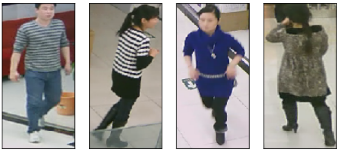
\includegraphics[width=13cm]{./content/images/sample_rapv1.png}
    \caption{Một số ảnh trong tập dữ liệu \textit{RAPv1}}
    \label{fig:sample-rapv1}
\end{figure}

\subsection{\texorpdfstring{Các thí nghiệm dự kiến sẽ triển khai}{Empty}}
Để hình thành ý tưởng và hoàn thành muc tiêu đã đề ra, cần nghiêm túc thực hiện các thí nghiệm liên quan tới các công trình đã được công bố. Một phần để kiểm chứng lại kết quả của công trình, một phần sẽ học tập được cách làm việc với môi trường của bài toán. Các thí nghiệm cần được triển khai:

$1$. Cài đặt và kiểm chứng bài báo của 
